\subsection{Hardware and Software selection} \label{subsec:soft}
% This subsection will outline hardware and software details used in the research process.
% It intended to provide necessary outlines to support further research and allow repeating the experiment with different conditions.

% Embedded devices for performance measurements
%
Three devices acted as embedded computing test units in different hardware and computational levels: Tensor Processing Unit (TPU), Raspberry Pi 4 (R-Pi4), and an Android-based smartphone.
Coral TPU produced by Google has limited specifications information, but the software has provided two libraries for average and maximum clock frequency computation.
Raspberry Pi 4 is powered with Quad-core Cortex-A72 (ARM v8) and 2GB RAM.
The Operating System was selected with a beta version of Raspbian 64 (aarch64).
The selection of Android devices depended on the highest percentage distribution.
An Octa-core Cortex-A53 with 3GB RAM seemed the most commonly used at the time.
The inbuilt chipset is Mediatek MT6753 (28 nm) with Android version 6.

% Model training Framework
%
The framework for Machine Learning has been Tensorflow 2.4.0 with Python 3.9.1 compiled from source using Bazel 3.1.0.
An additional package with Addons 0.18 for $R^2$ and Probability 0.13 for Differential Evoltions algorithms has been compiled from the source and added to the main framework.
Tensorboard is used to observe progress and keep records to analyse training later. It also made an excellent initial tool for model profiling and performance measure.

% Final performance tests
%
End of the training testing of each model has been performed on the Coral TPU device with TensorFlow-Lite Runtime library version 2.5.0.
Every model has been trained and converted to its' TFLite version to validate the ability to be suitable for deployment.
At the current stage and version of the TensorFlow, the Stateful models have not been supported for lite version conversion.
Final model testing against the entire set of all three profiles has been performed on a desktop machine with an Intel CPU and two Graphical Processors with Compute Capability Score of 7.5.
The version of the CUDA library for GPU computation that has been used is 11.1 from the beginning of the research.
%
% % IF
% \ifthenelse {\boolean{thesis}}
% %
% % THEN
% {
% \mbox{Figure~\ref{fig:device_compute}} demonstrates the paralysation mechanism for a single model, where flops and the total number of parameters are determined using the script in Appendix~\ref{app:flops}.
% }
% {
% \mbox{Figure~\ref{fig:device_compute}} demonstrates the paralysation mechanism for a single model version final testing, with three trained versions for each profile.
% }
% \begin{figure}[ht]
%     \centering
%     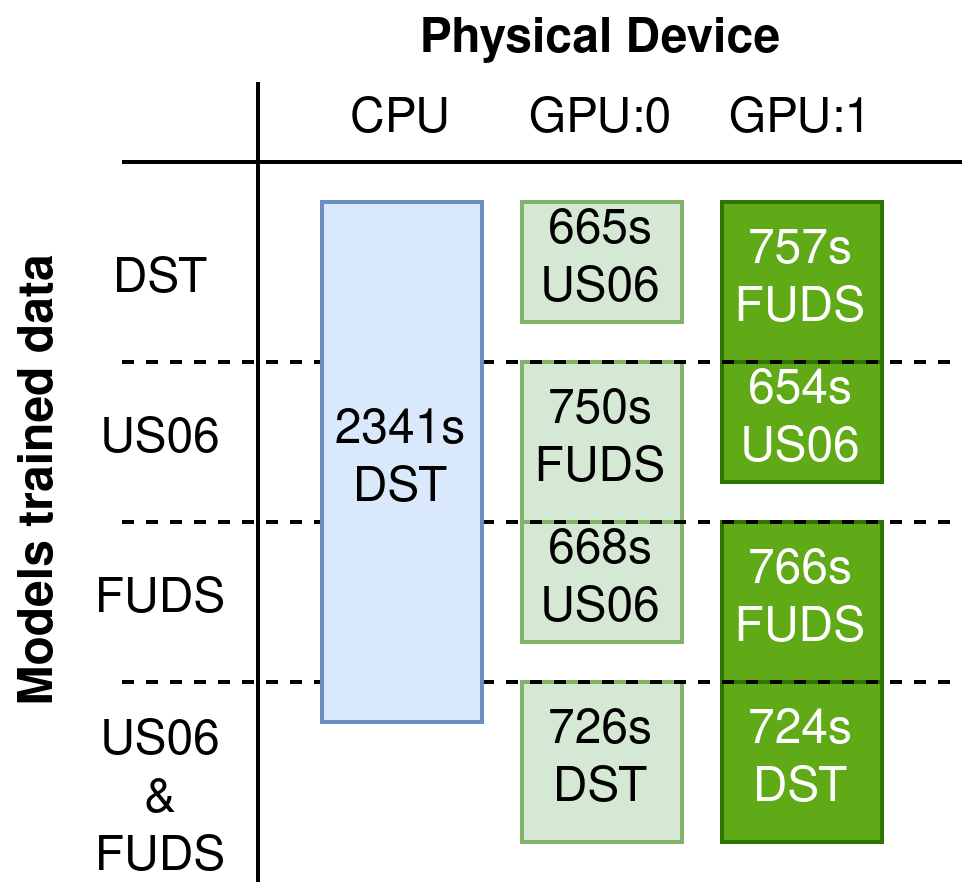
\includegraphics[width=\columnwidth]{II_Body/images/Accuracy_Compute.png}
%     % \includesvg[width=\linewidth]{II_Body/images/Accuracy_Compute_10.svg}
%     \caption{Accuracy computation using a single model trained on different proflies separately. The timing examples were taken from Model \#5 computation process.}
%     \label{fig:device_compute}
% \end{figure}
%
% Attention Layer has been reimplemented from provided source code.%\textcolor{red}{Good luck finding the link}
% Robust Adam was also implemented from the source; what should I do with that now?
% Multilayer model flagged with Return sequences boolean. Statefulnes define with Stateful boolean. The dropout is affected as a separate layer or parameter. With Stateful on, standard Input Layer shape requires to be follower Bacthed Input shape. It can be done kwarg parameter to the GRU or LSTM layer or kept as a separate Input Layer to allow precompilation before starting model fitting. Following code, the snipest demonstrated the difference. 

% \textcolor{red}{I am going to use the TPU processor to measure time it takes to run e ach model.} \\
% \begin{table}[ht]
%     \centering
%     \caption{Software details}
%     \label{tab:my_label}
%     \begin{tabular}{p{3.0cm}|c|c|c|c|c}
%         Version & Python version & Compiler & Build tools & CUDA version & Compute Score\\
%         Tensorflow-2.4.0, TF-Addons 13.0, TF-Probability 0.12.1 & 3.9.1 & gcc 9.3.0 & Bazel 3.1.0 & 11.1 & 7.5\\
%         \hline
%         Tensorflow-2.2.0 & 3.8.* & gcc 7.3.1 & Bazel 2.0.0 & CPU & 3.98MHz*
%     \end{tabular}
% \end{table}



%Table information collected as per datasheet. \\
%Android device: 3GB - RAM, Octa-core 1.3 GHz Cortex-A53, Android 5.1 (6), Chipset: Mediatek MT6753 (28 nm), \\

%GFLOPS table: http://web.eece.maine.edu/~vweaver/group/green_machines.html

% R-Pi3B as per Tim Chant:
% 70.45 GFLOPS / 6.2 GFLOPS/s = 11.36 s
% Total model flops / device flops = Time  --->>>>> Time * Device flops = Total model flops

% Energy consumption if Voltage and Current from device records not enough
% 1.36 s/s * 3.7 W / 3,600s = 0.0116 Wh/s


% \begin{table}[]
%     \centering
%     \caption{Chip-on-Board Hardware selection}
%     \label{tab:my_label}
%     \begin{tabular}{c|c|c|c}
%         Device & Specification & Source & Software setup \\
%         \hline
%         Coral TPU & (Specs) & (Link to the details) & (Link to libedgetpu.so.1) \\
%         \hline
%         Raspberry Pi 4 (Active cooling) & 
%     \end{tabular}
% \end{table}